% Author: Bernard Lampe

% Use the IEEE classes
\documentclass[journal]{IEEEtran}

% Packages
\usepackage[framed,numbered,autolinebreaks,useliterate]{mcode}
\usepackage[cmex10]{amsmath}
\usepackage{url}
\usepackage{cite}
\usepackage{graphicx}
\usepackage{subfig}
\usepackage{float}
\usepackage{bm}

% Correct bad hyphenation here
\hyphenation{op-tical net-works semi-conduc-tor}

% Start document
\begin{document}

% Paper title
\title{On Model Order Estimation by Information Theoretic Criteria}

% Author
\author{Bernard~Lampe,~\IEEEmembership{Member,~IEEE}}

% The paper headers
\markboth{Machine Learning for Signal Processing}
{Shell \MakeLowercase{\Lampe}: Machine Learning for Signal Processing}

% Make the title area
\maketitle

\begin{abstract}
Model order selection is an important first step when fitting a model to observed data. A very prolific method was developed by Wax and Kailath and is used widely for both model-driven and data-driven methods \cite{wax}. The solution put forth in their paper assumes a complex multivariate Gaussian model for the signal subspace and an isotropic Gaussian noise model for the noise subspace. In addition, they assume a linear mixture model of the signal subspace and noise subspace. With those assumptions they develop explicit Akaike Information Criteria (AIC) and minimum description length (MDL) and Bayesian Information Criteria (BIC) based estimators for selecting model order. In this study we investigate their formulation through empirical analysis with regard to estimator consistency and robustness to model mismatch.
\end{abstract}

% Keywords
\begin{IEEEkeywords}
Akaike Information Criterion, AIC, Minimum Description Language, MDL, Bayesian Information Criteria, BIC, Information Theoretic Criteria, ITC
\end{IEEEkeywords}

% Introduction with drop letter and first word capitalized.
\section{Introduction}
\IEEEPARstart{M}{odel} order selection is the focus of this study. In particular the formulation of information theoretic criteria to detect the number of signals. We follow the developments of Wax and Kailath \cite{wax} which is based on the the work of Akaike \cite{akaike}, Schwartz \cite{schwarz} and Rissanen \cite{rissanen}. In these works, they develop the Akaike Information Criteria (AIC), minimum description length (MDL) and Bayesian Information Criteria (BIC) to be used to detect the dimensionality of the signal subspace. We investigate these criteria empirically by implementing each in Matlab and observing the consistency and robustness of the estimators as the number of samples increases. Following what Wax and Kailath developed in their paper \cite{wax}, we use a stationary, ergodic and zero mean multivariate Gaussian random process for the signal subspace and isotropic multivariate Gaussian random process for the noise subspace.
\par The first step in the empirical investigation is to choose an appropriate mathematical formulation of the signal subspace and noise subspace. Following the procedure in \cite{liavas} and \cite{wax}, we assume a linear mixing model as in equation \ref{eq:mixing}. This equation decomposes the \(t\)-th observation, \(\bm{x}(t)\), as a linear combination of the \(q\) vectors in the signal subspace \(\{\bm{\alpha}_i\}_{i=1}^q\), where the scalars \(s_i(t)\) are the coefficients of the \(t\)-th signal and the vector \(\bm{n}(t)\) is the noise subspace vector at index \(t\). Where \(\bm{x}(t) \in I\!R^{p\text{x}1}\), \(\bm{\alpha}_i \in I\!R^{p\text{x}1}\), \(s_i(t) \in I\!R\) and \(\bm{n}(t) \in I\!R^{p\text{x}1}\).

\begin{equation}
\label{eq:mixing}
\bm{x}(t) = \sum_{i=1}^q \bm{\alpha}_i s_i(t) + \bm{n}(t)
\end{equation}

\par We can reformulate equation \ref{eq:mixing} to represent all \(N\) observations as in equation \ref{eq:all}. Here the observations are \(\bm{X} = [\bm{x}(1) | \bm{x}(2) | \dots | \bm{x}(N)]\), the signal subspace is \(\bm{A} = [\bm{\alpha}_1| \bm{\alpha}_2 | \dots | \bm{\alpha}_q]\), the signal coefficients are \(\bm{S} = [ \bm{s}(1) | \bm{s}(2) | \dots | \bm{s}(N)]\) and the noise is \(\bm{N} = [ \bm{n}(1) | \bm{n}(2) | \dots | \bm{n}(N) ]\). Where \(\bm{X} \in I\!R^{p\text{x}N}\), \(\bm{A} \in I\!R^{p\text{x}q}\), \(\bm{S} \in I\!R^{q\text{x}N}\) and \(\bm{N} \in I\!R^{p\text{x}N}\). We also assume the system in \ref{eq:all} is overdetermined, therefore \(q < p\).

\begin{equation}
\label{eq:all}
\bm{X} = \bm{A}\bm{S} + \bm{N}
\end{equation}

\par Our goal is to accurately determine the dimensionality of the signal subspace \(q\). If we assume that the signal subspace matrix \(\bm{A}\) is of full column rank, we can observe the eigenvalues of the correlation/covariance matrix of the data, denoted \(\bm{\lambda}^T = [\lambda_1, \lambda_2, \dots, \lambda_p] = \sigma(E\{\bm{X}\bm{X}^T\})\), to determine the dimension of the signal subspace. Where \(\lambda_1 > \lambda_2 > \dots > \lambda_p\). The first \(q\) eigenvalues attributed to the signal should be much larger than the \(p-q\) eigenvalues attributed to the noise if there is good signal to noise ratio in the data (SNR). In practice this approach is made difficult by the additive noise meaning the separation of "large" eigenvalues from "small" eigenvalues becomes ambiguous. In order to automate this process, Wax and Kailath purposed changing the eigenvalue detection problem into a model selection problem \cite{wax}. 

\subsection{AIC and MDL/BIC Criteria}
\par In order to convert the eigenvalue separation problem into a model selection problem, we need to select an appropriate statistical model \(f(\bm{X} | \bm{\Theta})\). Where \(\bm{X}\) is the observation matrix and \(\bm{\Theta}\) is the set of model parameters. Akaike proposed that the best fit model is the one with the minimum AIC \cite{akaike} as in equation \ref{eq:aic}. Schwartz and Rissanen proposed the minimum MDL and BIC respectively which turn out to be the same estimator in the limit of number of observations as in equation \ref{eq:mdl} \cite{rissanen}, \cite{schwarz}. Therefore, we consider MDL and BIC the same in this study. In each equation \(k\) is the evaluated model order. Both estimators, at the minimum, find the model order with the minimum Kulback-Liebler distance between the model density \(f(\bm{X}|\bm{\Theta})\) and the estimated model from the data \(f(\bm{X}|\hat{\bm{\Theta}})\). Each estimator consists of the maximum likelihood estimator (MLE) for the first term and a number of degrees of freedom term for the second term. Therefore, the first term will be relevant when fitting the data, and the second term will penalize a model which is too complex. The AIC tends to overestimate and not be as consistent as MDL/BIC. According to Wax and Kailath, any estimator with the form of \(-log(f(\bm{X}|\bm{\Theta})) + \alpha(N)k\) is consistent \cite{wax}. We can see that the second term of the AIC is not a function of \(N\) therefore the AIC tends to overestimate.

\begin{equation}
\label{eq:aic}
AIC(k) = -2 log(f(\bm{X} | \bm{\hat{\Theta}})) + 2k
\end{equation}

\begin{equation}
\label{eq:mdl}
MDL/BIC(k) = -log(f(\bm{X}|\bm{\hat{\Theta}})) + \frac{1}{2}klog(N)
\end{equation}

\par For this study, we follow the procedure in Wax and Kailath, and use a stationary, ergodic, zero-mean multivariate Gaussian distribution for the signal source. We also use a stationary, ergodic, zero-mean, isotropic multivariate Gaussian for the noise. Therefore, the covariance matrix for the noise component is \(\sigma^2I_{p\text{x}p}\) meaning the noise has the same variance in all directions and only one parameter is needed to account for the noise. Our sources of data are real numbers and not complex as was the development in Wax and Kailath. In order to appy the AIC and MDL/BIC criteria in equations \ref{eq:aic} and \ref{eq:mdl} we need to count the number of free model parameters for our real valued model. The number of parameters will be the number of degrees of freedom in the \(\bm{\hat{\Theta}}\) vector shown in equation \ref{eq:numparams}. There are \(k\) eigenvalues, 1 component for the isotropic noise variance and \(k\) eigenvectors. However, each eigenvector is normalized and orthogonal. Therefore, we lose \(k\) degrees of freedom for normalization and \(1/2k(k-1)\) degrees of freedom for orthogonalization. This means the number of degrees of freedom to estimate using the ITC is \(k + 1 + pk -k -1/2k(k-1) = k(p+1/2(1-k))+1\) degrees of freedom in total. If we apply the AIC and BIC/MDL criteria to the real valued Gaussian sources, we arrive at equations \ref{eq:aic_gauss} and \ref{eq:mdl_gauss}. Assuming the Gaussian model fits the data well, the minimum of the AIC/BIC/MDL functions will estimate the number of non-zero eigenvalues of the data such as equation \ref{eq:him}. We implemented both equations in Matlab and as a test arrived at the graphs in figures \ref{fig:fit_aic} and \ref{fig:fit_mdl}. This simple test confirmed our implementation by generating a 25 dimensional Gaussian with zero noise, high correlation and 1000 samples. We can see that this test chooses a conservative model order by looking at the eigenvalues of the data as in figure \ref{fig:eigs}. The AIC choose \(k^* = 18\) and MDL choose \(k^* = 15\). From the eigenvalue plot we can see that choice is just about when the curve flattens out completely.
\par If we study the equations in \ref{eq:aic_gauss} and \ref{eq:mdl_gauss}, we can see the first term is the log of the Gaussian MLE and the second term is the bias penalty term to keep the model from being too complex. The MLE terms are the ratio of the geometric mean to the arithmetic mean. There is a well known theorem that proves that the geometric mean is always less than or equal to the arithmetic mean with equality holding when all the values of \(l_i\) are equal to each other.  This means the first term will be zero if the data is isotropic and in the isotropic case, the AIC/MDL/BIC graphs will be parabolically increasing with respect to \(k\) giving \(k^*=1\). This is intuitively correct because there is only one non-zero eigenvalue with multiplicity \(p\). In other words, you only need to estimate the variance in one direction to know the variance in all directions in the isotropic case with no data correlation.

\begin{equation}
\label{eq:numparams}
\bm{\hat{\theta}} = (\lambda_1, \lambda_2, \dots, \lambda_k, \sigma^2, \bm{v}_1, \bm{v}_2, \dots, \bm{v}_k)
\end{equation}

\begin{align}
\begin{split}
\label{eq:aic_gauss}
AIC(k) = -2 &log\left(\frac{\prod_{i=k+1}^{p}l_i^{1/(p-k)}}{\frac{1}{p-k}\sum_{i = k+1}^{p}l_i} \right)^{(p-k)N} \\
       &+ 2k(p+\frac{1}{2}(1-k)) + 1
\end{split}
\end{align}

\begin{align}
\begin{split}
\label{eq:mdl_gauss}
MDL/BIC(k) = - &log\left(\frac{\prod_{i=k+1}^{p}l_i^{1/(p-k)}}{\frac{1}{p-k}\sum_{i = k+1}^{p}l_i} \right)^{(p-k)N} \\
       &+ \frac{1}{2} (k(p+\frac{1}{2}(1-k))+1)log(N)
\end{split}
\end{align}

\begin{align}
\begin{split}
\label{eq:him}
\hat{k}^* &= \min_{0<k<p-1}(AIC/MDL/BIC(k)) \\
          & \approx |\{\lambda_1, \lambda_2, \dots, \lambda_q, \sigma^2, \bm{v}_1, \bm{v}_2, \dots, \bm{v}_k\}|.
\end{split}
\end{align}

\begin{figure}[h]
\centering
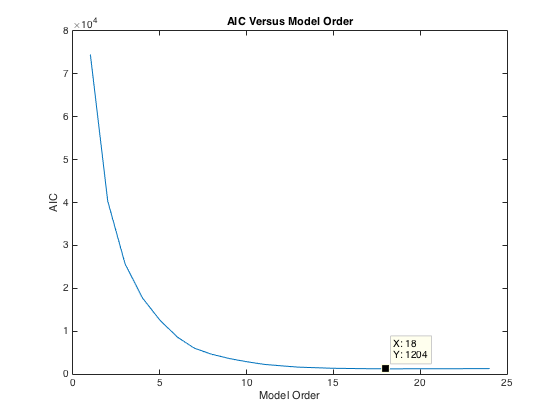
\includegraphics[width=3.1in]{../images/model_fit_example_aic_25_099_1000.png}
\caption{AIC Curve for multivariate Gaussian \(p=25\), Correlation \(\rho = 0.99\) and \(1000\) Samples. Minimum is annotated at \(k^* = 18\).}
\label{fig:fit_aic}
\end{figure}

\begin{figure}[h]
\centering
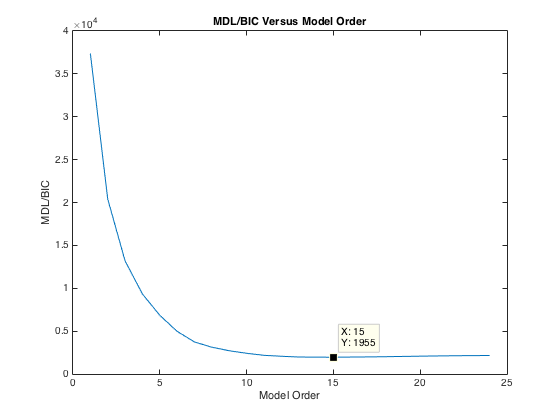
\includegraphics[width=3.1in]{../images/model_fit_example_mdl_25_099_1000.png}
\caption{MDL Curve for multivariate Gaussian \(p=25\), Correlation \(\rho = 0.99\) and \(1000\) Samples. Minimum is annotated at \(k^* = 15\).}
\label{fig:fit_mdl}
\end{figure}

\begin{figure}[h!]
\centering
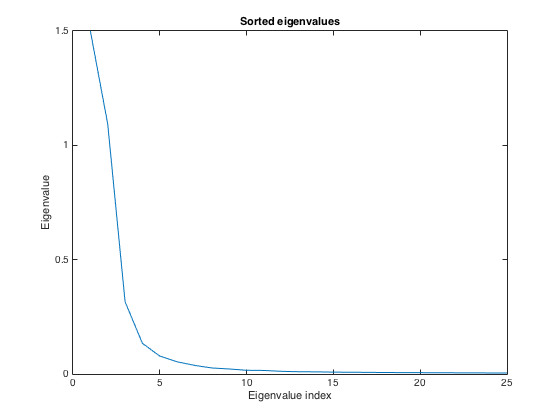
\includegraphics[width=3.1in]{../images/eigs.png}
\caption{Zoomed in plot of Eigenvalues for multivariate Gaussian \(p = 25\), Correlation \(\rho = 0.99\) and \(1000\) samples.}
\label{fig:eigs}
\end{figure}

\section{Data Generation}
\par In order to generate test data for our empirical study we use the multivariate generalized power exponential family of distributions from the paper by Gomez, et. al. \cite{gomez}. We reproduce the equation for data generation from their paper in equations \ref{eq:mggd} and \ref{eq:mggd_k}. The equation is parameterized by \(\bm{\Theta} = \{\bm{u}, \bm{\Sigma}, \bm{\beta}\}\) where we set the mean \(\bm{u} = \bm{0}\). We also have an algorithmic way to compute \(\bm{\Sigma}\) where the covariance values are a function of the distance from the center diagonal which is parameterized by \(\rho\). If \(\rho = 0\), then \(\bm{\Sigma} = I_{p\text{x}p}\) and there is no correlation in the data and the data is isotropic. If, we increase \(\rho > 0\) then the correlation increases with an exponential decay off the diagonal. Figure \ref{fig:covariance} is a surface plot for \(\bm{\Sigma}\) when the dimension of the data is \(p = 50\) and the correlation parameter \(\rho = 0.99\). Also, figure \ref{fig:hist_r_085_b_1} shows the resulting Gaussian with correlation \(\rho = 0.85\). Finally, if \(\beta = 1\), then the data generated is Gaussian distributed. There is an example of this for 2 dimensional data in figure \ref{fig:hist_b_1}. If \(\beta < 1\), then the generated data becomes super Gaussian where the kurtosis increases beyond 3. There is an example of super Gaussian for 2 dimensional data in figure \ref{fig:hist_b_01}.  If \(\beta > 1\), then the data becomes sub Gaussian where the kurtosis decreases below 3. An example of sub Gaussian for 2 dimensional data is in figure \ref{fig:hist_b_100}. For robustness testing, we vary the kurtosis in order to make the data non-Gaussian. In addition, we decided to try two other multivariate distributions. The first was random and the second was a Beta distribution with the parameters \(\alpha = \beta = 0.5\). This Beta distribution disperses the density to the tails of the distribution making it highly non-Gaussian. An example of the Beta distribution in 2 dimensions is in figure \ref{fig:beta_dist}.

\begin{align}
\begin{split}
\label{eq:mggd}
f(\bm{x}; \bm{u}, \bm{\Sigma}, \bm{\beta}) &= \\
    k|\Sigma|^{-\frac{1}{2}}&\exp{\left\{-\frac{1}{2}[(\bm{x} - \bm{u})^H\Sigma^{-1}(\bm{x}-\bm{u})]^{\beta}\right\}}
\end{split}
\end{align}

\begin{align}
\begin{split}
\label{eq:mggd_k}
k = \frac{n\Gamma(\frac{n}{2})}{\pi^{\frac{n}{2}} \Gamma(1 + \frac{n}{2\beta})2^{1+\frac{n}{2\beta}}}
\end{split}
\end{align}

\begin{figure}[h]
\centering
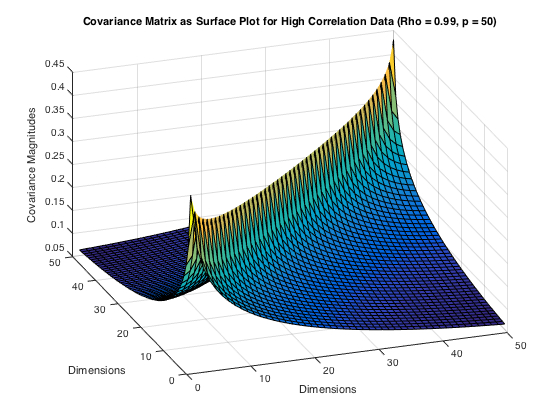
\includegraphics[width=3.1in]{../images/covariance.png}
\caption{Surface Plot of Covariance Matrix of High Dimension Gaussian Data Generation Model Using \(p = 50, \rho = 0.99, \beta = 1\)}
\label{fig:covariance}
\end{figure}

\begin{figure}[h]
\centering
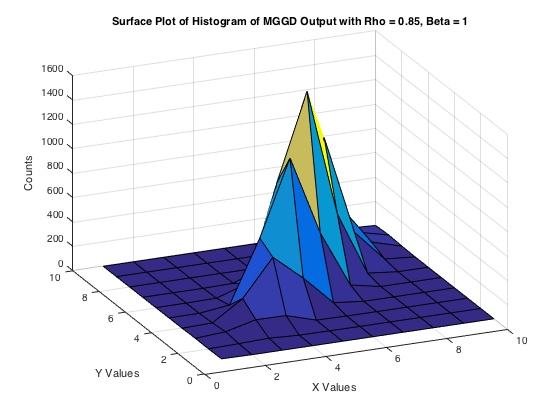
\includegraphics[width=3.1in]{../images/hist_r_085_b_1.png}
\caption{Surface Plot of Histogram With \(p = 2\), \(\rho = 0.85\), \(\beta = 1\), \(10,000\) samples}
\label{fig:hist_r_085_b_1}
\end{figure}

\begin{figure}[h]
\centering
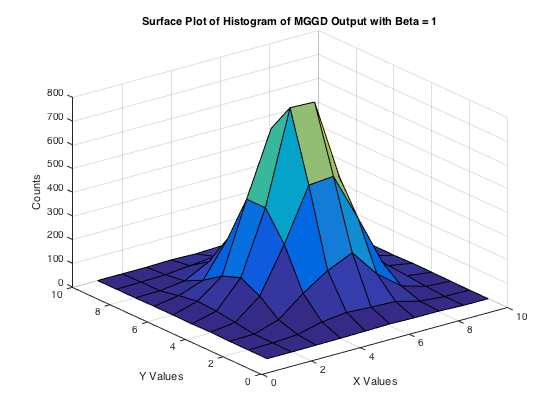
\includegraphics[width=3.1in]{../images/hist_b_1.png}
\caption{Surface Plot of Histogram With \(p = 2\), \(\rho = 0\), \(\beta = 1\), \(10,000\) samples}
\label{fig:hist_b_1}
\end{figure}

\begin{figure}[h]
\centering
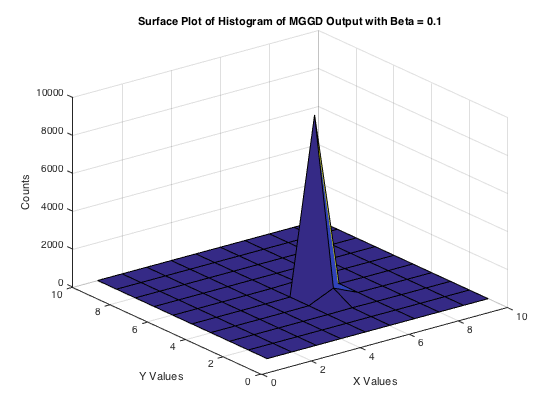
\includegraphics[width=3.1in]{../images/hist_b_01.png}
\caption{Surface Plot of Histogram With \(p = 2\), \(\rho = 0\), \(\beta = 0.1\), \(10,000\) samples}
\label{fig:hist_b_01}
\end{figure}

\begin{figure}[h]
\centering
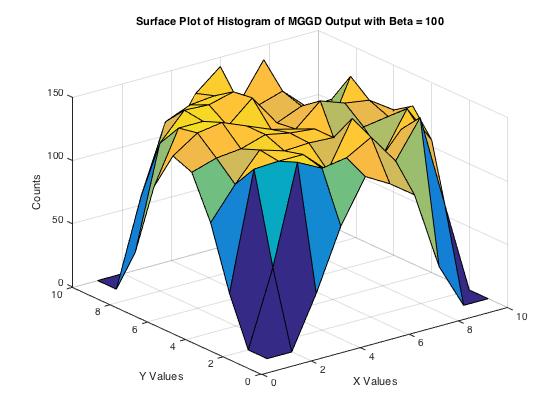
\includegraphics[width=3.1in]{../images/hist_b_100.png}
\caption{Surface Plot of Histogram With \(p = 2\), \(\rho = 0\), \(\beta = 100\), \(10,000\) samples}
\label{fig:hist_b_100}
\end{figure}

\begin{figure}[h]
\centering
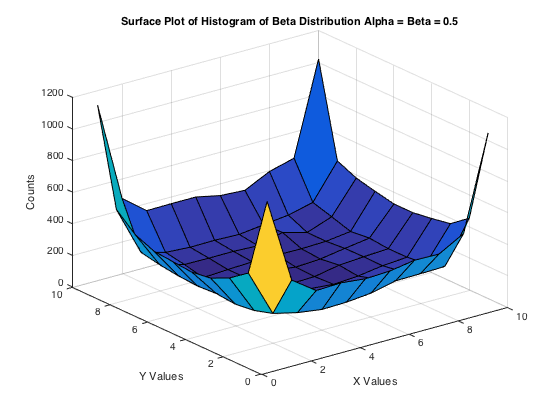
\includegraphics[width=3.1in]{../images/hist_beta_05_05.png}
\caption{Surface Plot of Histogram of Beta Distribution \(p = 2\), \(\alpha = \beta = 0.5\)}
\label{fig:beta_dist}
\end{figure}

\section{Experiments}
\par For all experiments, we generated the entire data set only once meaning that for the experiment where the sample size \(N\) varies, we generate the data and then take subsets of that data. This was done so that we can see how adding IID samples to the same set of samples changes the AIC and MDL/BIC. If you generate the data on each run for increasing samples sizes, the graphs of the model selection criteria are harder to draw conclusions from. This experimental design choice does not change the conclusions which could be drawn, but makes them more apparent in the graphs.

\subsection{Consistency of Criteria}
\par We conducted several experiments to determine how the AIC and MDL/BIC criteria performed when increasing the number of samples. The first experiment was with a model order of \(p = 25\) with a minimum of 25 to 25,000 samples. The second experiment was with a model order of \(p = 50\) and 50 to 50,000 samples. Both the experiments were conducted with \(\beta = 1\) meaning that we generated Gaussian data to match the assumed model. Our goal is to investigate the consistency of AIC/MDL/BIC as the number of samples increases, how correlation effects the criteria and how the dimensionality of the data effects the criteria. Also, we are concerned with how AIC compares with MDL/BIC in regards to convergence and consistency. The graphs for experiment one are in figures \ref{fig:aiccon25} and \ref{fig:mdlcon25}. The graphs for experiment two are in figures \ref{fig:aiccon50} and \ref{fig:mdlcon50}.

\begin{figure}[h]
\centering
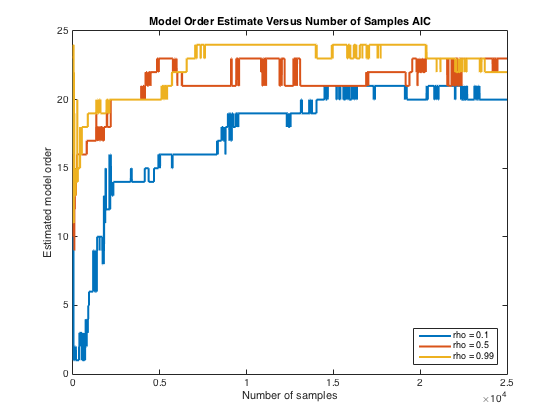
\includegraphics[width=3.1in]{../images/consistency_aic_rho_25.png}
\caption{AIC Model Order Estimate Versus Number of Samples for Lower Dimensional Model \(p = 25\), \(\beta = 1\), \(N = 25\) to \(25,000\) and Varying Correlation}
\label{fig:aiccon25}
\end{figure}

\begin{figure}[h]
\centering
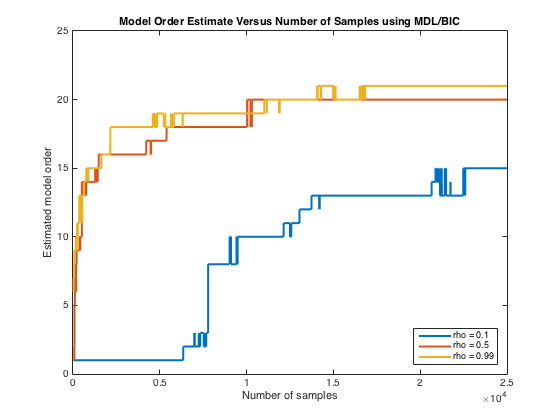
\includegraphics[width=3.1in]{../images/consistency_mdl_rho_25.png}
\caption{MDL Model Order Estimate Versus Number of Samples for Lower Dimensional Model \(p = 25\), \(\beta = 1\), \(N = 25\) to \(25,000\) and Varying Correlation}
\label{fig:mdlcon25}
\end{figure}

\begin{figure}[h]
\centering
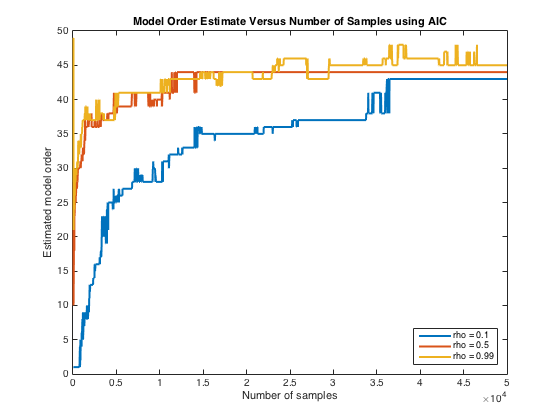
\includegraphics[width=3.1in]{../images/consistency_aic_rho_50.png}
\caption{AIC Model Order Estimate Versus Number of Samples for Higher Dimensional Model \(p = 50\), \(\beta = 1\), \(N = 50\) to \(50,000\) and Varying Correlation}
\label{fig:aiccon50}
\end{figure}

\begin{figure}[h]
\centering
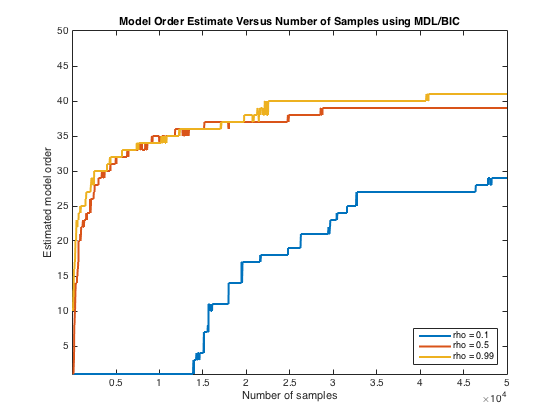
\includegraphics[width=3.1in]{../images/consistency_mdl_rho_50.png}
\caption{MDL Model Order Estimate Versus Number of Samples for Higher Dimensional Model \(p = 50\), \(\beta = 1\), \(N = 50\) to \(50,000\) and Varying Correlation}
\label{fig:mdlcon50}
\end{figure}

\subsection{Robustness from Gaussian Assumption}
\par We conducted more experiments to determine how the AIC and MDL/BIC criteria performed when the underlying data violates the Gaussian assumed model. In these experiments we fix \(p = 25\), the number of samples varies from \(N = 25\) to \(25,000\) and \(\rho = \{0.1, 0.99\}\) for both high and low correlation. We examine the behavior of the AIC/MDL/BIC criteria when the number of samples increases and the correlation parameter for data generation in equation \ref{eq:mggd}, \(\beta\), is not 1. Therefore, we are introducing higher and lower kurtosis into the generated data. The graphs for these experiments are in figures \ref{fig:aicdev01}, \ref{fig:mdldev01}, \ref{fig:aicdev99} and \ref{fig:mdldev99}. We did two different \(\rho = \{0.1, 0.99\}\) values to determine if correlation had an effect when the model assumption was violated. In addition, we generated data using a Random distribution and a Beta distribution to study an example of other distributions which are highly non-Gaussian. The Random and Beta distributions we generated were symmetric and therefore the Gaussian it fit was always isotropic, therefore \(k^*\) was always 1 meaning there was no correlation in the Gaussian data. This is why we did not graph the results of those test.

\begin{figure}[h]
\centering
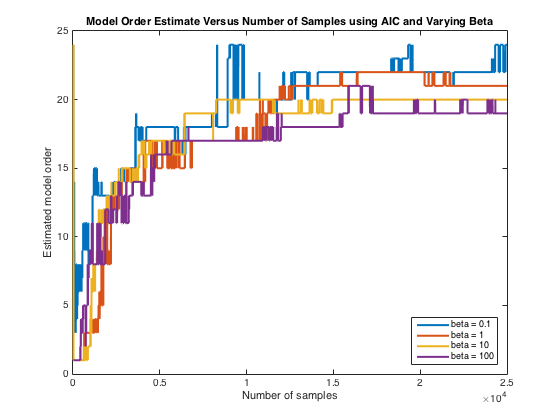
\includegraphics[width=3.1in]{../images/deviation_aic_01.png}
\caption{AIC Model Order Estimate Versus Number of Samples for Lower Dimensional Model \(p = 25\), Lower Correlation \(\rho = 0.1\), \(N = 25\) to \(25,000\) and Varying Beta \(\beta = {0.1, 1, 10, 100}\).}
\label{fig:aicdev01}
\end{figure}

\begin{figure}[h]
\centering
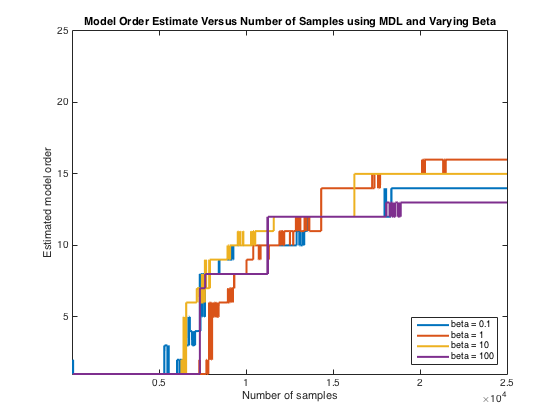
\includegraphics[width=3.1in]{../images/deviation_mdl_01.png}
\caption{MDL Model Order Estimate Versus Number of Samples for Lower Dimensional Model \(p = 25\), Lower Correlation \(\rho = 0.1\), \(N = 25\) to \(25,000\) and Varying Beta \(\beta = {0.1, 1, 10, 100}\).}
\label{fig:mdldev01}
\end{figure}

\begin{figure}[h]
\centering
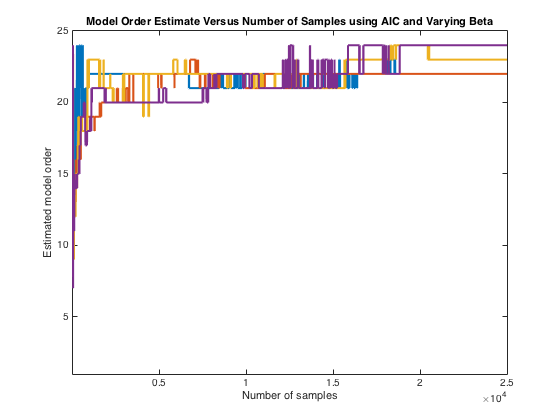
\includegraphics[width=3.1in]{../images/deviation_aic_099.png}
\caption{AIC Model Order Estimate Versus Number of Samples for Lower Dimensional Model \(p = 25\), Higher Correlation \(\rho = 0.99\), \(N = 25\) to \(25,000\) and Varying Beta \(\beta = {0.1, 1, 10, 100}\).}
\label{fig:aicdev99}
\end{figure}

\begin{figure}[h]
\centering
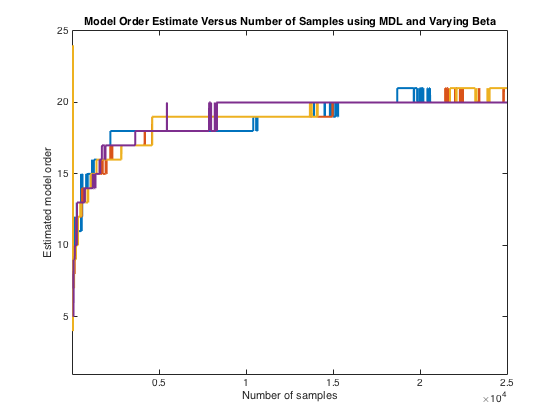
\includegraphics[width=3.1in]{../images/deviation_mdl_099.png}
\caption{MDL Model Order Estimate Versus Number of Samples for Lower Dimensional Model \(p = 25\), Higher Correlation \(\rho = 0.99\), \(N = 25\) to \(25,000\) and Varying Beta \(\beta = {0.1, 1, 10, 100}\).}
\label{fig:mdldev99}
\end{figure}


\section{Conclusions}
\subsection{Consistency as Number of Samples Increases}
\par From the first experiment where we generate Gaussian data with parameters of \(p = 25, \beta = 1, N = [25, 25000]\) for both AIC and MDL/BIC in figures \ref{fig:aiccon25} and \ref{fig:mdlcon25}, we can see that the AIC overestimates when compared to MDL/BIC which was sited as a problem in the Wax and Kailath paper \cite{wax}. We also see that the AIC has more variability in the limit as \(N \to \infty\). We expect some variability because the estimators converge in probability. Therefore, when we run enough tests we should see some fluctuation. However the AIC seems to fluctuate more with compared to MDL/BIC. In addition, we can clearly see that the lower the correlation in the data, the more samples that are required for all the criteria to converge. For example, the blue curves in figures \ref{fig:aiccon25} and \ref{fig:mdlcon25} are low correlation and certainly take many more samples to converge and in the MDL case the low correlation data did not converge to the correct solution in \(25,000\) samples. This is because the number of samples needed to characterize the low correlation data by the eigenvalues of the covariance matrix is considerable due to the eigenvalues being close in value to each other and random fluctuations will interfere with convergence. In contrast, the highly correlated data converges quite quickly in comparison. We also see the trend that AIC converges faster than the MDL/BIC criteria. However, this is at the cost of variability and overestimation trend mentioned before. AIC captures more subtle correlations in the data faster, but if there are too few samples, the AIC is unreliable which is shown when there are very few samples and the AIC graph peaks to a value of \(p\).
\par We were also interest in how the dimensionality of the data samples effected the convergence and therefore, we ran the same experiment using \(p = 50, \beta = 1, N = [25, 25000]\). The results are graphed in figures \ref{fig:aiccon50} and \ref{fig:mdlcon50}. We see the same trends as the first experiment but with one added observation that the number of samples needed for the model selection criteria to converge when doubling the dimensionality increases considerably. This is intuitive and follows the well known curse of dimensionality problem. As we increase the dimension of the data, we need an exponential number of samples for the statistics computed from the data to converge.

\subsection{Robustness as Gaussian Assumption is Violated}
\par The next experiment we ran was to change the generated data away from a Gaussian to a sub and super Gaussian by modifying kurtosis away from 3. The results are graphed for both a low correlation case, in figures \ref{fig:aicdev01} and \ref{fig:mdldev01}, and a high correlation case \ref{fig:aicdev99} and \ref{fig:mdldev99}. From the graphs for the lower correlation, you can see that as we change the \(\beta\) parameter away from 1, the estimates for the model order tend to vary considerably. When \(\beta = 1\) the data is Gaussian and we were sure to plot the Gaussian case with the Non-Gaussian cases. As you can see there is more fluctuation, but the estimator does not deviate wildly. This is attributed to the fact that we are still generating data which is from the Gaussian family. In the highly correlated data experiment in figures \ref{fig:aicdev99} and \ref{fig:mdldev99} we see just as before that the model selection criteria converges faster and we again see the fluctuations as in the lower correlation Non-Gaussian experiment. However, there is one new observation in figure \ref{fig:mdldev99}. If you look at the graph closely, you can see that when there are few samples and high correlation, the MDL/BIC criteria varies widely. This is because we don't have enough samples and the Non-Gaussian data is not generating data that is isotropic. Therefore, the MDL/BIC may compute a very high model order erroneously as it did in this case.
\par We also compute graphs for the AIC and MDL/BIC criteria with a random distribution and a symmetric Beta distribution. However, we did not provide the resulting graphs here because the output of both AIC and MDL/BIC was a constant 1. This is because the Gaussian model we assumed was trying to fit symmetric data, which means the Gaussian that best fit was isotropic. Clearly this is an inadequate model as the KL distance between a Gaussian and Random or Beta distribution is very high and a model order of 1 would not suffice to capture any of the underlying signals. We conclude that the model selection criteria in this paper is inadequate if the data is significantly different that the assumed model and the criteria can vary wildly if the data is undersampled and this is especially bad in higher dimensional models and samples.

% References section
\nocite{*}
\bibliographystyle{plain}
\bibliography{./references}

% Biography
\begin{IEEEbiographynophoto}{Bernard Lampe}
(M'09) became an IEEE Member (M) in 2009 and received his bachelors of science degree from The University of Michigan in Ann Arbor, Michigan, USA in 2009.
\par Mr. Lampe is also a member of the American Society for Computing Machines (ACM) since 2009.
\end{IEEEbiographynophoto}

% matlab code
\begin{lstlisting}
function [aic, mdl] = model_order(data)

% data: observations vectors assumings each row is a vector
% K: max model order to compute
% return: aic, bic and mdl information criteria vectors for 1:K model order

% compute the correlation matrix
[p, n] = size(data);
R = data * data'./n;

% compute the eigenvectors
e = sort(eig(R), 'descend');

% compute information criteria for all possible k = 1:p-1
aic = zeros(p-1, 1);
mdl = zeros(p-1, 1);
for k = 1:p-1
    aic(k) = gauss_aic(e(k+1:p), k, n, p);
    mdl(k) = gauss_mdl(e(k+1:p), k, n, p);
end

% aic function
function aic = gauss_aic(l, k, n, p)
    aic = -2 * (p-k) * n * log(geomean(l) / mean(l)) + 2 * k * (p + 0.5 * (1 - k)) + 1
end

% mdl function
function mdl = gauss_mdl(l, k, n, p)
    mdl = -(p-k) * n * log(geomean(l) / mean(l)) + 0.5 * k * (k * (p + 0.5 * (1-k)) + 1) * log(n);
end

end
\end{lstlisting}

% End document
\end{document}

